\documentclass[a4paper]{article}
\usepackage{graphicx}
\usepackage{hyperref}
\usepackage{authblk}

\title{Semi-automatic staging area to feed SuperCon with high-quality structured data from scientific literature}
\author[1,2]{Luca Foppiano}
\author[1]{Tomoya Mato}
\author[3]{Kensei Terashima}
\author[4]{Pedro Ortiz Suarez}
\author[3]{Tou Taku}
\author[3]{Chikako Sakai}
\author[3]{Wei-Sheng Wang}
\author[2]{Toshiyuki Amagasa}
\author[3]{Takano Yoshihiko}
\author[1]{Ishii Masashi}
\affil[1]{Materials Modelling Group, Data-driven Materials Research Field, Centre for Basic Research on Materials, NIMS, Japan}
\affil[2]{Knowledge and Data Engineering, Centre for Computational Sciences, University of Tsukuba, Japan}
\affil[3]{Frontier Superconducting Materials Group, MANA, NIMS, Tsukuba, Japan}
\affil[4]{DFKI GmbH, Germany}

\begin{document}

\maketitle

\begin{abstract}
    TBA
\end{abstract}

\section{Introduction}

The emergence of new statistical methodologies in machine learning for materials exploration has given rise to a burgeoning research area called materials informatics (MI) ~\cite{10.3389/fchem.2022.930369}.
This field focuses on the exploration of functional materials and aims to efficiently screen materials with desired properties by leveraging the materials data accumulated in the past.
As a matter of course, this approach requires a larger number of material-related data for training models.
Researchers have been developing large aggregated databases of physical properties generated by first principles calculations based on density functional theory (DFT), such as Materials Project~\cite{materialsprojectJain2013}, JARVIS~\cite{aflowcurtarolo2012aflow}, NOMAD~\cite{nomad}, and so on, that played a role of a solid driving force for the development of materials informatics.
However, such DFT-based physical property values are not necessarily always be valid, since they are derived by a certain approximation of many-body interactions in solids.
Therefore, applicability of such calculated data is still challenging for building a machine-learned model of complicated physical properties like superconductivity.
Despite the rapid growth in scientific publications, including exponential raise in materials science~\cite{Pratheepan_2019}, there is a scarcity of accumulated datasets of experimental data. 
The limited resources available, such as the Pauling File~\cite{Blokhin2018ThePF_paulingFile} and SuperCon~\cite{SuperCon}, has resulted in the reliance on manual extraction methods.
This could be attributed to the lack of adequate infrastructures and expertise in the field.

% The lack of adequate infrastructures and expertise could have leaded to create a single manual procedure that can extract information from diverse sources like plots, tables, and text all at once. However, while this approach may be viable in the short term, its sustainability diminishes over time. 
% On the other hand, constructing an automated process to accomplish this task presents many challenges. In the case of scientific publications, plots, tables, and text necessitates different treatments, and the resulting outputs must be merged and verified manually. Despite the challenges, it is possible to transition gradually towards automation by implementing iterative steps. This iterative approach involves reducing human involvement progressively while simultaneously optimising the efficiency of required human actions. 

SuperCon~\cite{SuperCon} was built manually over more than a decade by the National Institute for Materials Science (NIMS) in Japan and it is considered the gold standard in superconductors research.
Despite being praised for its excellent quality in numerous reports~\cite{roter2020predicting, stanev_machine_2017, tran2022machine, konno2021deep}, the updates of SuperCon have become increasingly challenging due to the high publication rate. However, in response to the need for a more efficient approach to sustain productivity, we embarked on the development of an automated system for extracting material and property information from text contained in relevant scientific publications~\cite{lfoppiano2023automatic}. This automated process enabled the rapid creation of SuperCon2, a comprehensive database of superconductors containing over 35,000 entries, within an operation duration of just a few days. 

Ensuring the same quality as SuperCon while automating the extraction of structured superconductors data poses significant challenges. 
We developed a web interface designed to facilitate the curation process, involving the active and ongoing management of data through its lifecycle of interest, specifically tailored for our superconductors database but open to potential adaptation other data structures. 
Our interface aims to maintain quality, add value, and provide for reuse over time while making the curation process faster, more effective, and user-friendly.

There are several tools for data annotation, such as Inception~\cite{klie-etal-2018-inception}, Doccano~\cite{doccano}, at the moment of writing this article, we are not aware of any other curation tools for materials extracted databases. 
This paper introduces our curation tool, SuperCon2, which serves as a data staging area for SuperCon. The tool allows for the visualisation, correction, and integration of automatically extracted data into the SuperCon database, while triggering a feedback loop to improve the machine learning (ML) models.

Our contributions in this work are as follows:
\begin{itemize}
    \item We designed an efficient and scalable ingestion process for processing batches of PDF documents,
    \item We designed a lightweight anomaly detection process for fast outliers identification, 
    \item We present a new interface designed for data curation in materials science, 
    \item We integrate the visualisation of the extracted materials-related entities with the PDF document viewer. This utilises coordinates extracted by Grobid~\cite{GROBID}, and it was demonstrated in other fields by~\cite{wang2022hammer}. [Add more references] 
    \item We establish a feedback loop mechanism that generates training data at the sentence level based on the data correction process.
\end{itemize}

The subsequent sections of this paper elaborate on the interface and its design principles, the ingestion and corrections processes. Finally, we present some results from the feedback loop. 

\section{User interface}

The SuperCon2 curation interface offers several key features to facilitate the data curation process.

It provides a comprehensive view that visualises materials and their related properties as a table which includes search, filtering, and sorting functionality (Figure~\ref{fig:curation-interface-database}). 
The schema consists of two main classes: material information (material names, formulas, shape, etc.) and properties (T\textsubscript{c}, applied pressure, measurement method, etc.). The complete list including examples is reported in our previous work~\cite{lfoppiano2023automatic}.

\begin{figure}[t]
  \centering
  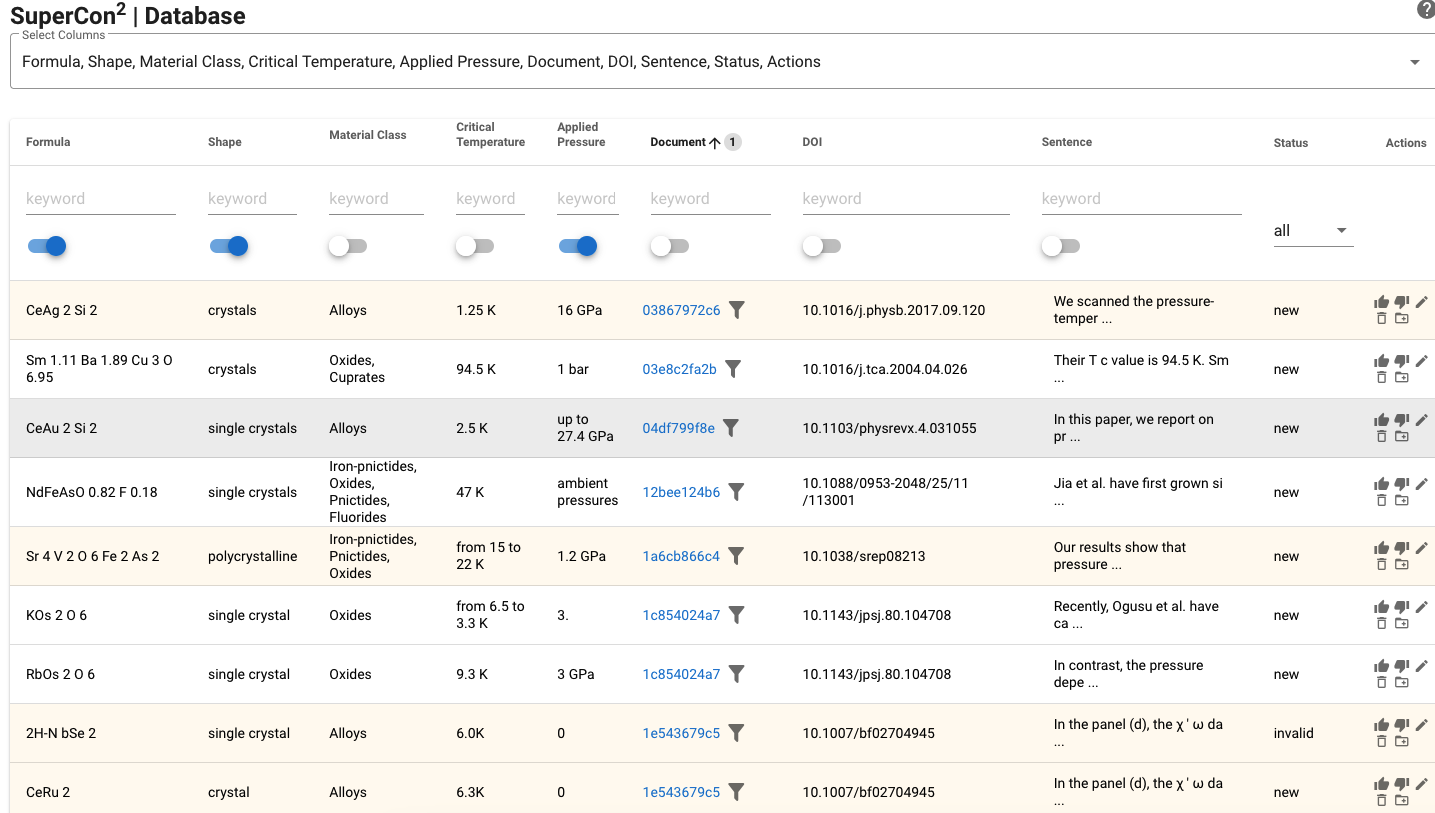
\includegraphics[width=1\textwidth]{images/supercon-curation-database} 
  \caption{Curation interface showing the database as a table}
  \label{fig:curation-interface-database}
\end{figure}


During the curation process is often necessary to navigate back and forth to the related section to the extracted record that is being examined. The curation interface provides a document viewer combining a table with the extracted records and the viewer of their respective document (Figure~\ref{fig:pdf-view}). The viewer highlights the annotations that identify materials and properties, enabling users to easily locate and reference the extracted information within the document.

Each record presented can be modified, removed, or flagged. The flagging was built with the idea of having two phases of curation: in the first phase, the records are examined quickly mostly without checking the document information, and the users flags any record that judge incorrect. In the second step, slower, the user goes through the invalid information and examine them thoughtfully correcting when needed and stepping back to the document to check the context. 

The interface automatically collects training data. When a record is corrected, the information pertaining to the sentence, spans (annotations), and tokens (including layout information, fonts, and other features) is gathered, enabling the generation of valuable training data for further improvements in the automated extraction process.

\begin{figure}[ht]
  \centering
  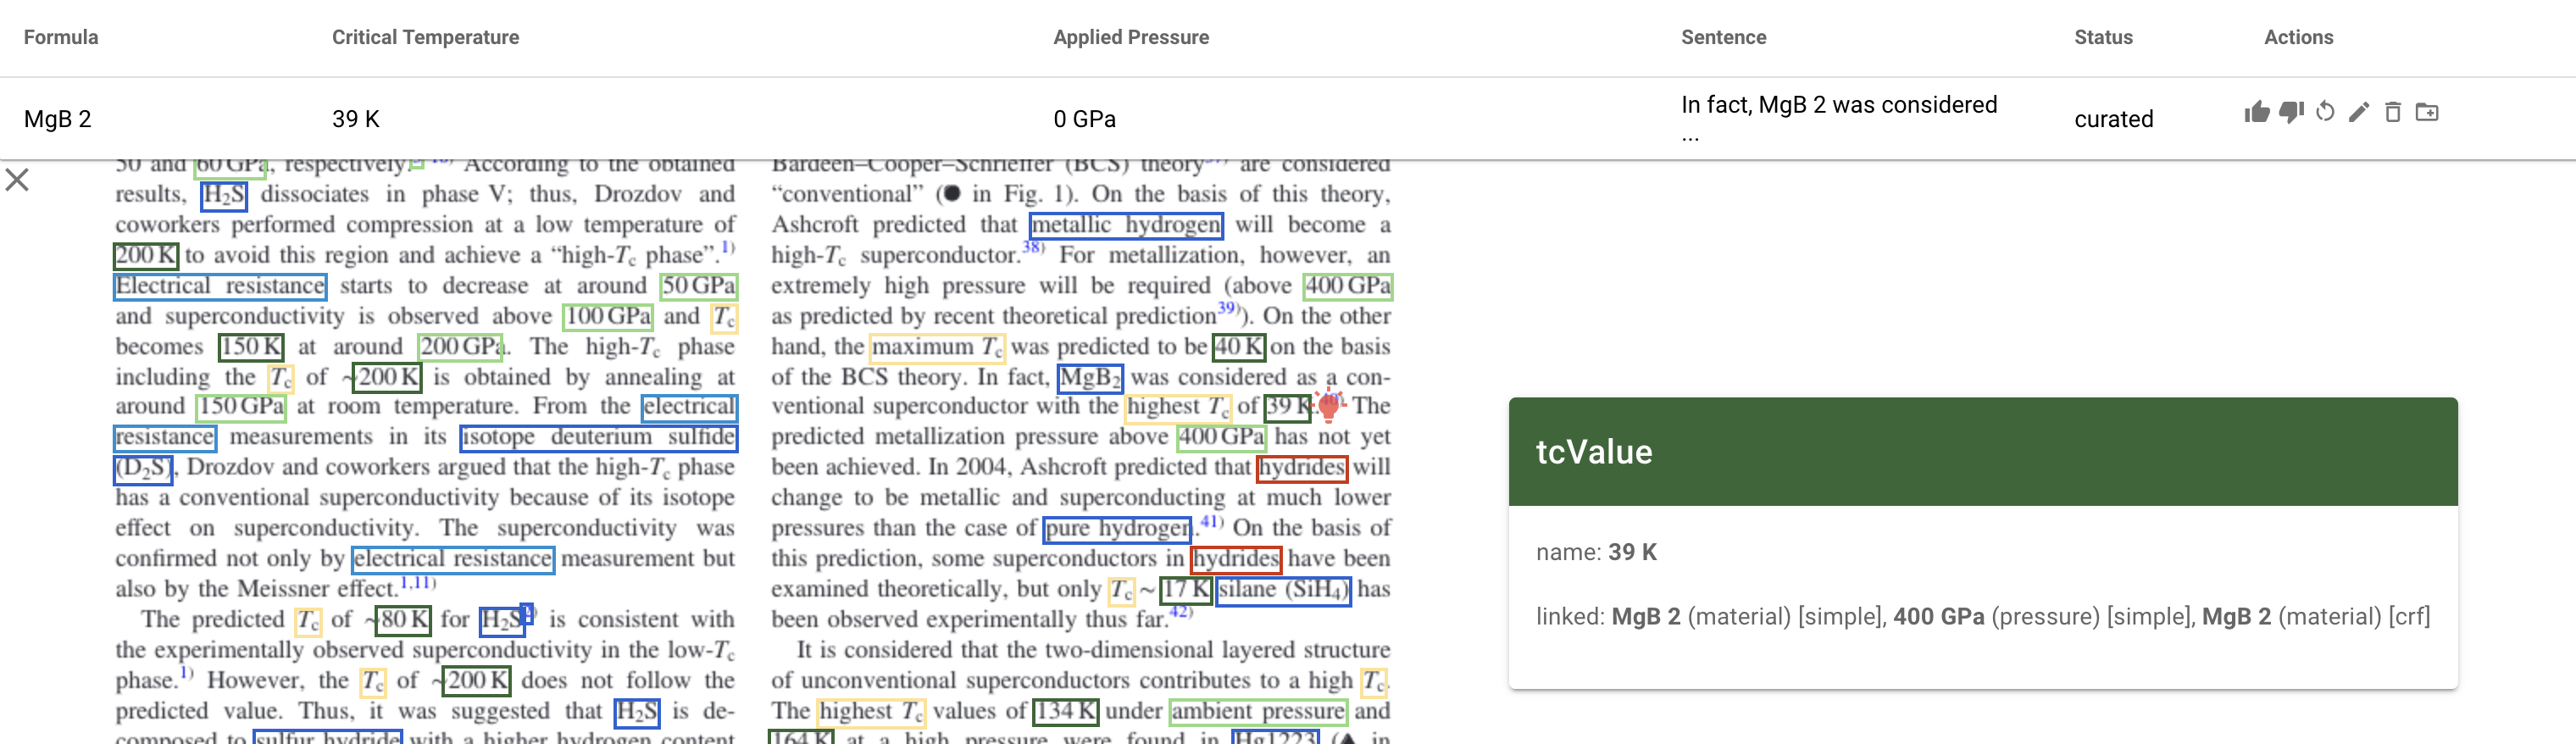
\includegraphics[width=1\textwidth]{images/pdf-view-context.png} 
  \caption{PDF document viewer showing an annotated document. The table on top is linked through the annotated entities. The user can navigate from the record to the exact point in the PDF, with a pointer (the red bulb light) identifying the context of the entities being examined. }
  \label{fig:pdf-view}
\end{figure}

% \begin{figure}[ht]
%   \centering
%   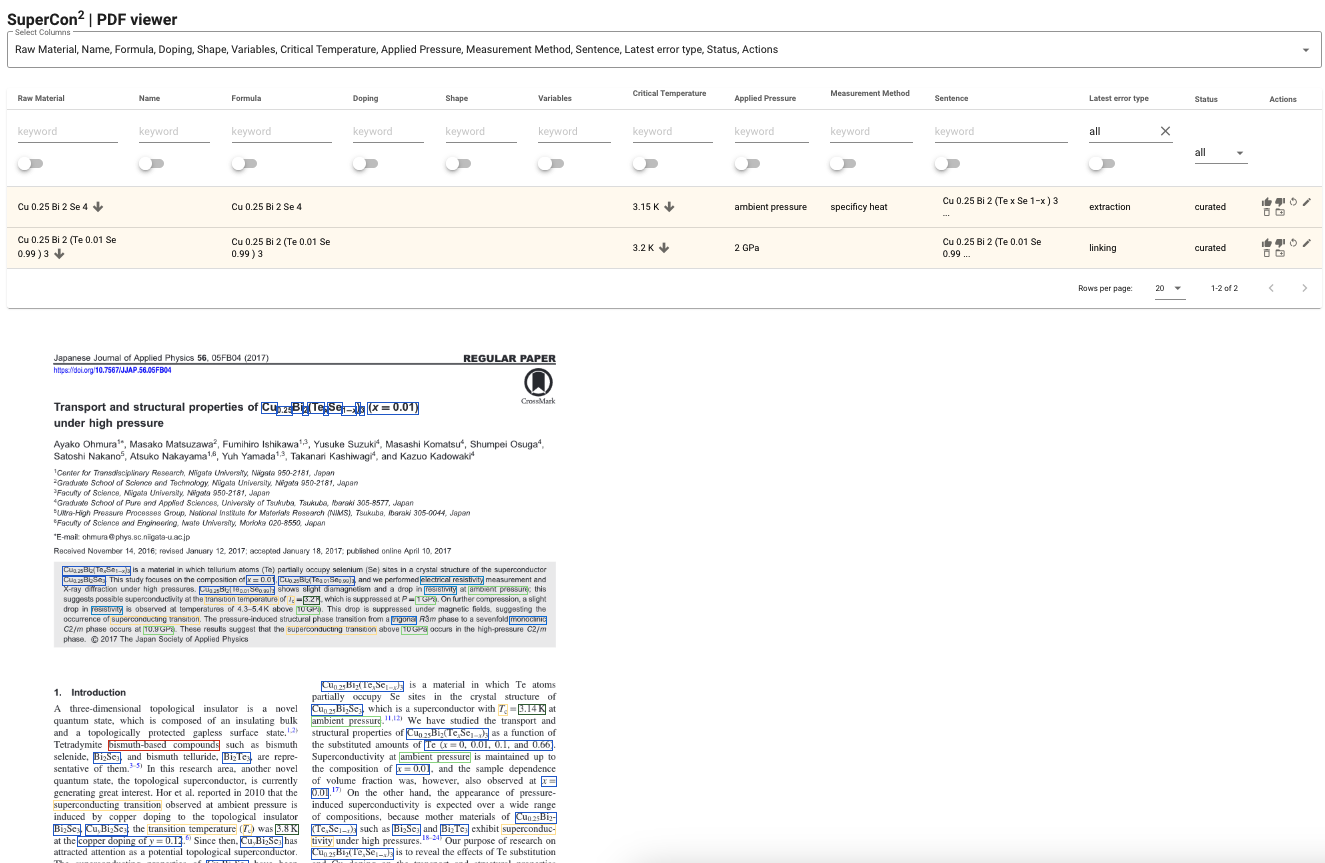
\includegraphics[width=1\textwidth]{images/supercon-curation-pdf-viewer} 
%   \caption{PDF viewer. The page includes a table showcasing records extracted from the  current document, along with the PDF content and accompanying annotations.}
%   \label{fig:curation-interface-pdf-viewer}
% \end{figure}


\subsection{Data flow and model}
\label{subsec:data-flow}

The data flow is first introduced in our previous work~\cite{lfoppiano2023automatic} using a Map-Reduce approach. 
First, in the "extraction task", the PDF documents are stored and processed by grobid-superconductors which transform them in the corresponding annotations format. The format is illustrated in Figure~\ref{fig:data-flow-2} and is structured as a list of "passages" (sentences or paragraphs). 

\begin{figure}[ht]
  \centering
  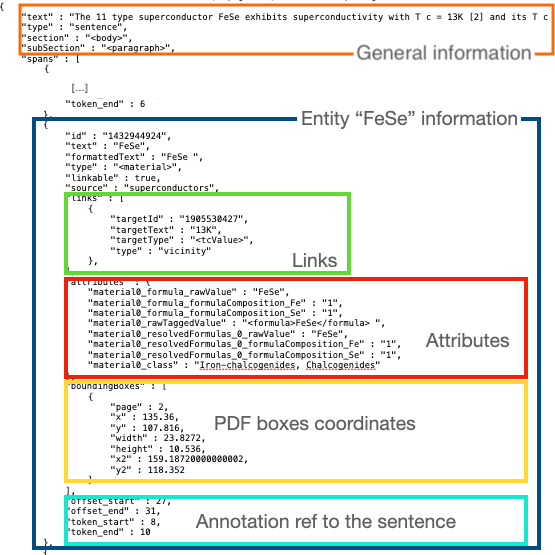
\includegraphics[width=0.8\textwidth]{images/data-flow-2} 
  \caption{Example of a passage extracted in the "extraction task". We highlight the different structured information in a single span: links, attributes, PDF coordinates (to visualise annotations on the PDF document), and annotations references within the sentence (to visualise annotations on text).}
  \label{fig:data-flow-2}
\end{figure}

Each passage is composed of the following attributes: the text of the passage, the type, of passage (sentence or paragraph), the main section: header, body, and annex, and the subsections: title, abstract, paragraph, caption. 
Furthermore, there is the list of spans containing the extracted entities which include the text, type, attributes, the tokens containing layout information (font size, font face, superscript, subscript, bold, italic, coordinates), a unique identifier, and other internal information (source ML model) and whether is allowed to be linked (temperatures not classified as superconductors critical temperatures are set to linkable = False).
The attributes are stored as a key-value and mainly contain information extracted by the material parser: the formula, the structured composition, and the material class.  

Second, in the "aggregation task", the annotated documents are aggregated as flat table format, of which each row becomes a \textit{record} of one material and its properties. For materials containing more information, for example, when the paper describes different doping ratio, the records are duplicated and the non-variable attributes are copied. 
% In Figure~\ref{fig:data-flow-3} there is an example of flat table record. 

% \begin{figure}
  % \centering
  % 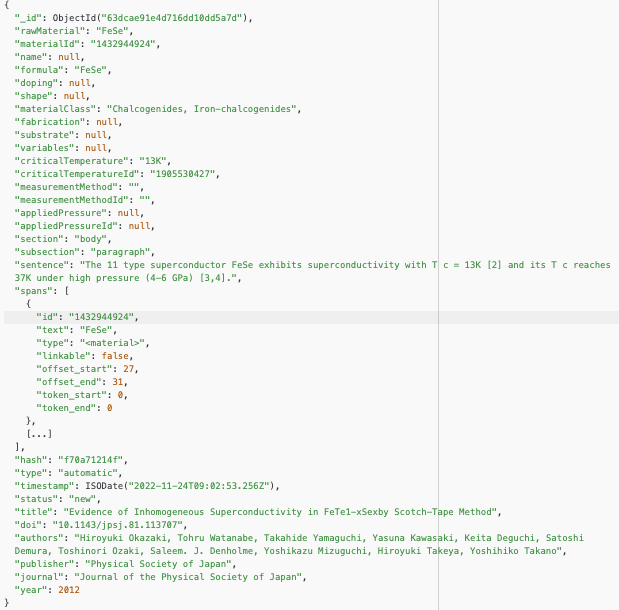
\includegraphics[width=0.8\textwidth]{images/data-flow-3} 
  % \caption{Example of record after the aggregation.)}
  % \label{fig:data-flow-3}
% \end{figure}

\subsection{Design principles}
\label{subsec:design-principles}

The design principle is a set of rules we chose at the beginning of the development. 

\paragraph{Blind correction}
This interface has been built without any multi-user mechanism. 
The data is allocated to different curators by generating randomised links to the application. Each link opens records extracted from a specific document. 
The justification for this approach is twofold: a) the allocation is totally random and each curation does not know any information about the others, and b) the multi-user implementation requires a large effort without any particular scientific gain. 

\paragraph{Data-driven architecture} When a record is modified its data is duplicated and a new record is created. 
This, allows us now to collect curation records knowing which data was corrected, and when and how many changes were done. In future, this feature will simplify the implementation of the undo/redo operations. 
When a record is deleted, its status is modified to "removed", and the record is hidden. 

On the contrary, binary records, such as PDF documents, are not duplicated, for saving disk space. Obviously, this does not forbid loading two different PDF documents of the same article, because the hash code would be different. In such cases the anomaly detection (Section~\ref{subsec:anomaly-detection} will notice the duplication and report it. 

The PDF documents binary content is used to generate a hash code of 8 character which is used to avoid duplicated PDF documents, for linking documents and records within the database. Each record, and even each span have its own unique identifier which are calculated using the span attributes.

\begin{figure}[ht]
  \centering
  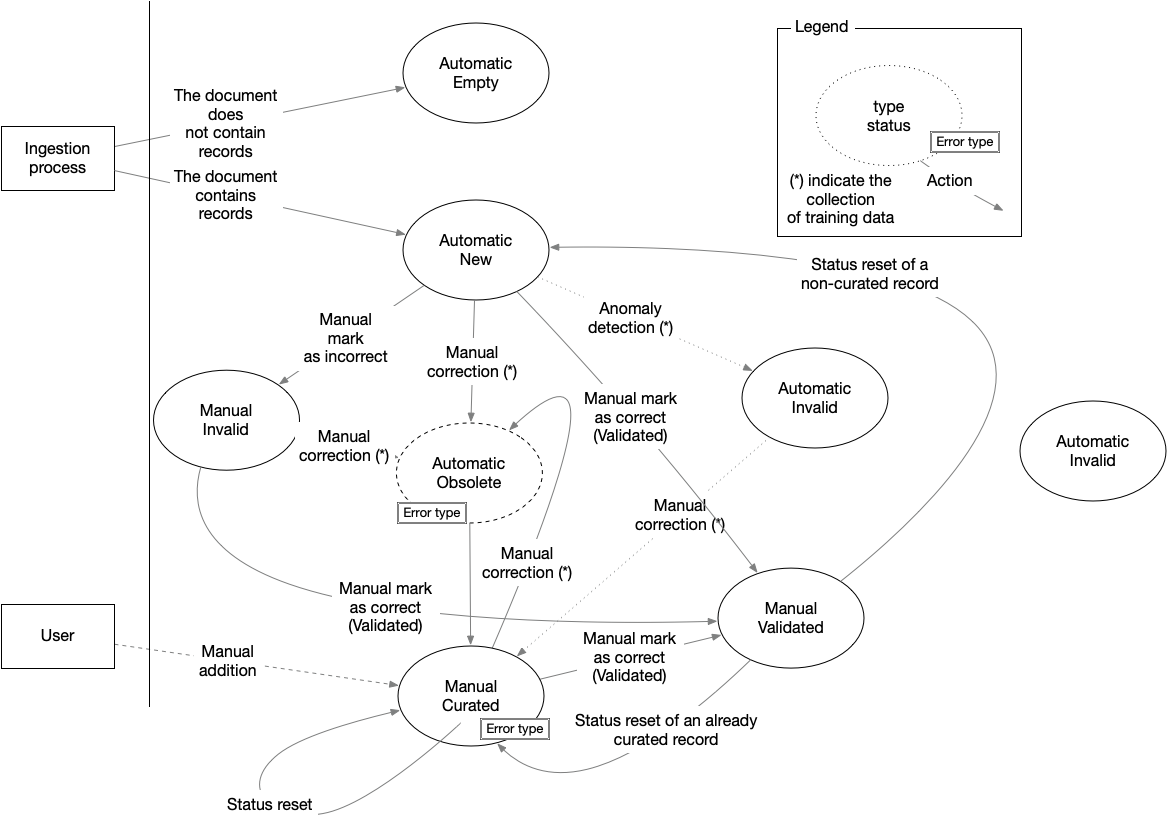
\includegraphics[width=1\textwidth]{images/record-correction} 
  \caption{Schema of the curation workflow. Each state is characterised by two properties: type and status, and one action, as indicated in the top right corner. "Error type" indicates the action of storing the error type for that specific action.}
  \label{fig:curation-workflow}
\end{figure}

\paragraph{Type and Status} Each \textit{record} has two workflow-related fields which are combined to identify the state of the workflow, which is illustrated in Figure~\ref{fig:curation-workflow}. 
The status indicates the record curation status from the data point of view, and is summarised in Table~\ref{tab:record-status}

\begin{table}[htbp]
\centering
\begin{tabular}{|p{2cm}|p{10cm}|}
\hline
\textbf{Status} & \textbf{Description} \\
\hline
new & Default status when a new record is created. \\
\hline
curated & The record has been updated by a human. \\
\hline
validated & The record was validated by a human. \\
\hline
invalid & The record is wrong or inappropriate for the situation (e.g., Tm or Tcurie extracted as superconducting critical temperature). \\
\hline
obsolete & Assigned to a record when it is modified, triggering the creation of a new record (internal status, not visible to users).\\
\hline
deleted & The record has been removed by a curator (internal status, not visible to users). \\
\hline
\end{tabular}
\caption{Record status definitions}
\label{tab:record-status}
\end{table}
    
The type indicates whether the record has been created or modified manually or automatically. The value "automatic" is provided when the data is loaded and/or when the anomaly detection performs some operations. All other cases it is flipped to "manual". 

\paragraph{Error types} Error types were first introduced in~\cite{lfoppiano2023automatic} while performing manually the end-to-end evaluation. They were combined with the evaluation to provide more detailed information on the reasons why certain extracted values were not correct. 
Since such statistics demonstrated to be useful during the development, we have extended the scope to add additional values related to data curation and validation (Table~\ref{tab:error-types}).

\begin{table}[htbp]
\centering
\begin{tabular}{|p{4cm}|p{8cm}|}
\hline
\textbf{Name} & \textbf{Description} \\
\hline
From table & The entities Material $\rightarrow$ Tc $\rightarrow$ Pressure are identified in a table. At the moment, table extraction is not performed. \\
\hline
Extraction & The material, temperature, pressure are not extracted (no box) or extracted incorrectly. \\
\hline
Linking & The material is incorrectly linked to the Tc given that the entities are correctly recognized. \\
\hline
Tc classification & The temperature is not correctly classified as "superconductors critical temperature" (e.g., Curie temperature, Magnetic temperature...). \\
\hline
Composition resolution & The exact composition cannot be resolved (e.g., the stoichiometric values cannot be resolved). \\
\hline
Value resolution & The extracted formula contains variables that cannot be resolved, even after having read the paper. This includes when data is from tables. \\
\hline
Anomaly detection & The data is automatically modified by the anomaly detection script. \\
\hline
Curation amend & The curator is updating the data which does not present issues due to the automatic system. \\
\hline
\end{tabular}
\caption{Summary of error type values and description.}
\label{tab:error-types}
\end{table}

In the curation interface we made the error type mandatory at each modification, including deletion as well. Since often the modifications are not related to a mistake, e.g. adding a space in a formula to make it more clear, or replacing garbled characters, we allow an additional error type called "Curation amend" which indicate that the problem is not related to the automatic system. This covers also the case where the modification corrects a mistake from another curator. 
When the updated is made, a new record is created, and the error type is stored in the previous record. The workflow schema in Figure~\ref{fig:curation-workflow} indicate "error type" in the states that requires it's selection. 

\subsubsection{Usability}
The usability is an important aspect in evaluating an interface. 
The criteria for evaluating the usability of a user interface can vary depending on the context and specific goals of the evaluation. 
In regard to SuperCon\textsuperscript{2}, the simplicity makes it easier to evaluate, considering the main requirement being smoothly transition between the database records and the context in the document. 
We consider the WEBUSE (WEBsite USability Evaluation Tool)~\cite{chiew2003webuse} evaluation criteria for our analysis. WEBUSE has been considered for evaluating web pages usability in many works and it can be summarised as follows: 
\begin{itemize}
    \item Content, organisation, and readability. The usability of a user interface can be evaluated based on how well the content is presented (clear and concise information) and organised (logical organisation), and how easily readable it is. 
    \item Navigation and links. The ease of navigation and the effectiveness of links within the user interface are important criteria for usability evaluation. 
    \item User interface design. The interface should be visually pleasing and visually consistent throughout the application or website. 
    \item Performance and effectiveness. Performance and efficiency in making the users achieving their goals.
\end{itemize}

We discuss the four criteria as follows. 
\paragraph{Content, organisation and readability} The interface is simple and organised in two main pages: database and document. Since the database contains many columns we have reduced the ones visible by default, to make the table fitting in the average screen. We use colours to separate records belonging to different documents. 

\paragraph{Navigation and links} The interface was designed with a minimalist approach. 
There are links and shortcuts in many duplicated positions to reduce the effort for certain repeated actions.
Finally, we provide an alternative and more efficient approach to navigation and correction using only the keyboard. 

\paragraph{User interface design}
The user interface utilises Vue.js, a modern JavaScript framework, enabling reactive operations such as text input and filtering. Additionally, it adopts the Vuetify design framework, which adheres to Google's recommended Material Design principles, ensuring a consistent visual design.

\paragraph{Performance and effectiveness}
We designed the transitions to reduce the time required by users to lookup the text from the record. 
One way is to visualise in the table view, the sentence the record is contained in, decorated with coloured spans to identify the annotations. This aims to provide users a quick check of the context without the original layout. 
The second approach is to point to the related part of the PDF document decorated with the extracted annotations (Figure~\ref{fig:pdf-view}). In this way, curator will increase their productivity by reducing the time spent in the tedious task of searching for information in the PDF document. 
 
We designed an experiment to measure the effectiveness of the user interface, as compared with the traditional approach. 
We selected X (X=6?) papers and distributed to a pool of 2 curators. For each paper we provided the PDF document to one curator and the processed version through the interface to the second curator. We measured the time required by each curator has to extract the relevant information. 
At each paper iteration we swapped the means (document vs interface) to randomise the experiment. 

We found out that... 


\subsubsection{Curation and processing logs}

The Supercon\textsuperscript{2} interface records minimal information regarding the ingestion (processing log) and the curation process (curation log). 
The processing log is filled-up when the data is ingested, it was build to have minimal functions able to explain why certain documents haven't been processed (Figure~\ref{fig:processing-curation-log}). 
Grobid was built focusing on speed and robustness, and contains several fail-safe mechanisms to avoid crashing the system when a document is either too big or does not contains valuable information, for example does not have any text. Old PDF documents (e.g. before 1990) are likely have been scanned and contains only images. 
Examples of too big documents are dissertation thesis with more than 100 pages, that might be collected by mistake. 


\begin{figure}[ht]
  \centering
  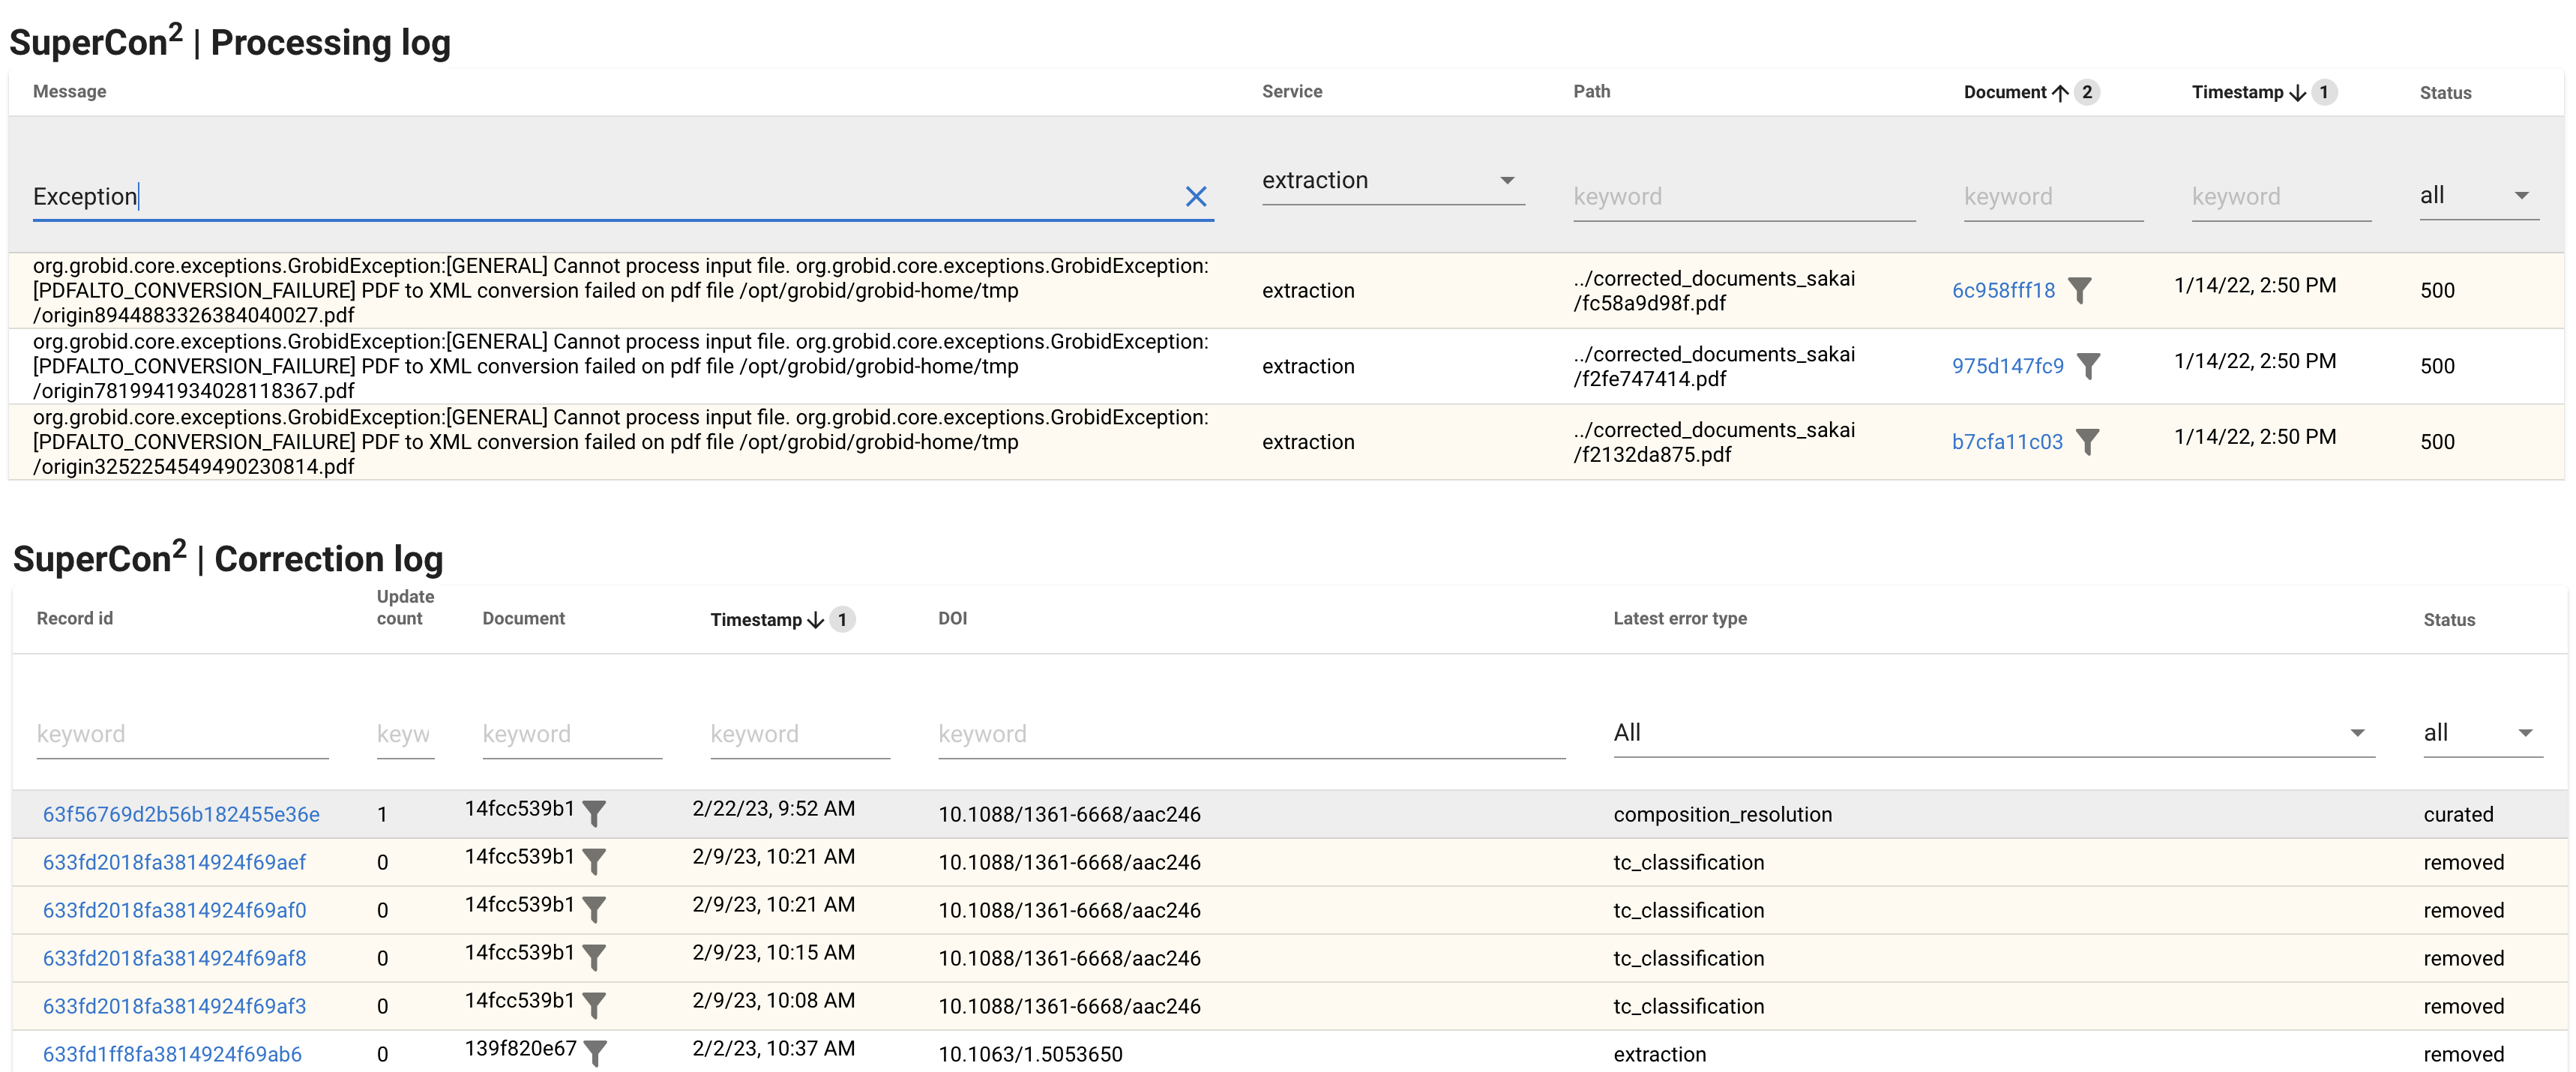
\includegraphics[width=1\textwidth]{images/processing-curation-log.png} 
  \caption{On the top: Processing log, showing the output of each operation (process document, create record) and the outcome with the exception or error should have occurred. On the bottom: Curation log, indicating each record, the number of updates, and the date/time of the last updates.}
  \label{fig:processing-curation-log}
\end{figure}

The curation log provide a view on the corrections that are performed in an aggregated page. 
The curation log shows all the records that have been updated and when. It includes also the history of each record (Figure~\ref{fig:processing-curation-log}).

% \begin{figure}[ht]
%   \centering
%   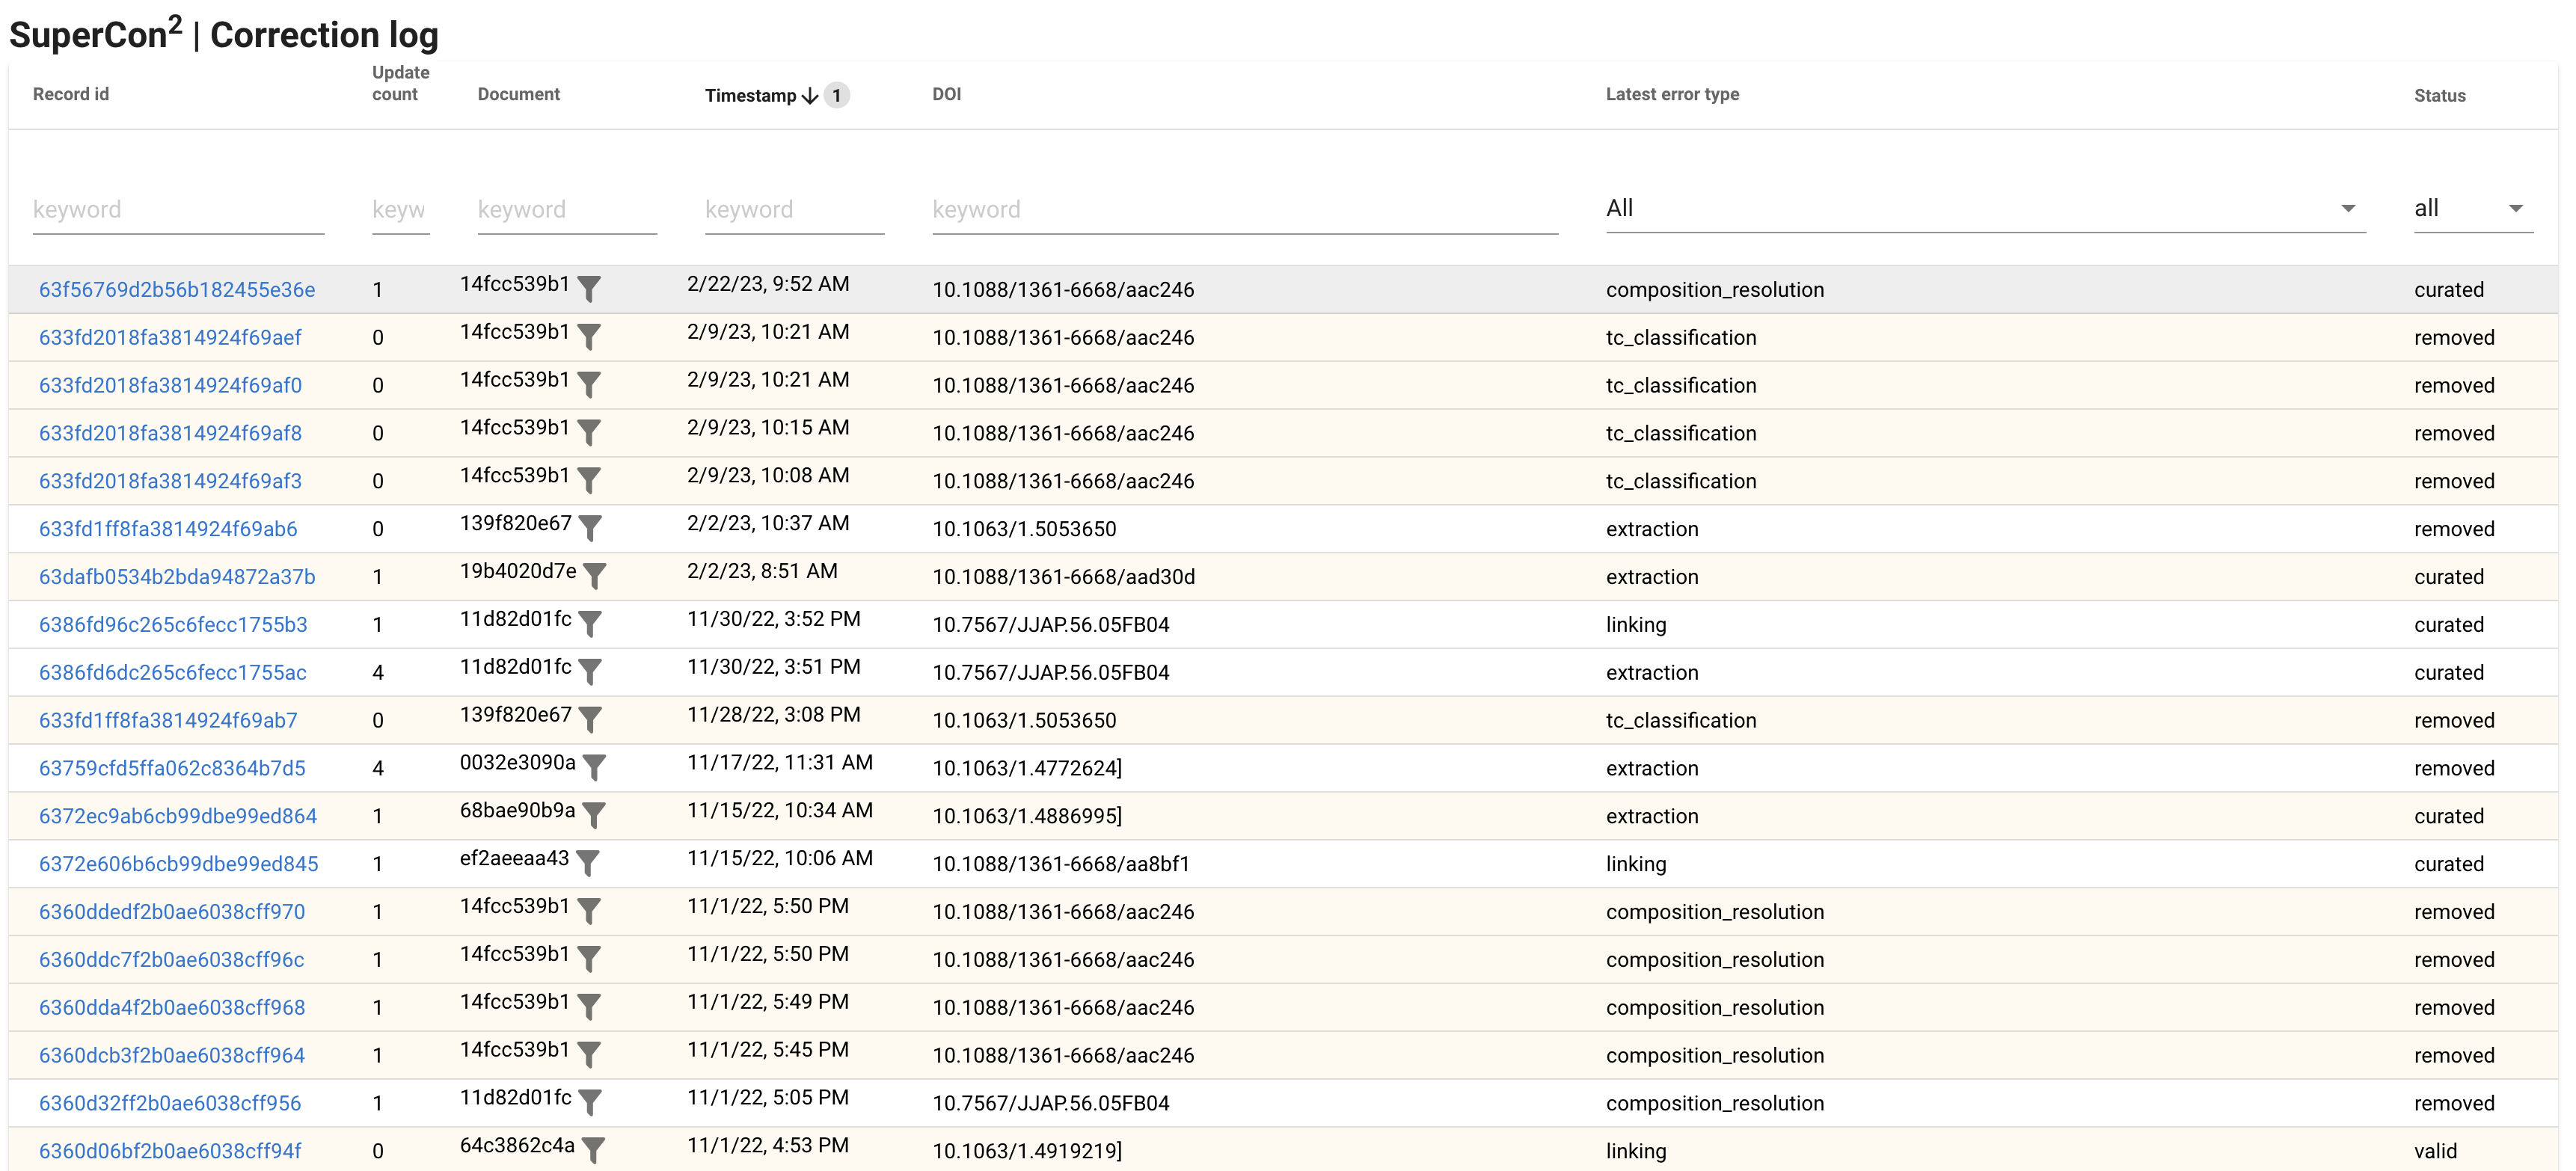
\includegraphics[width=1\textwidth]{images/curation-log} 
%   \caption{Curation log, indicating each record, the number of updates, and the date/time of the last updates. }
%   \label{fig:curation-log}
% \end{figure}


\section{Data correction for automatically extracted entities in SuperCon\textsuperscript{2}}
In this section we describe the processes related to data correction using the user interface. 
In Section~\ref{subsec:anomaly-detection} we discuss anomaly detection as the pre-processing phase, since the extracted data from grobid-superconductors may contains mistakes.
Then, the core phase, the manual correction process is described in Section~\ref{subsec:manual_correction}. We employ only domain-experts as curators in order to certify the correctness of the data outcome. 
At each correction, we collect potential training data to be utilised as feedback loop for the trained ML model, which is covered in Section~\ref{subsec:feedback-loop-training-data}.

\subsection{Anomaly detection}
\label{subsec:anomaly-detection}
Anomaly detection is the process of identifying unusual or unexpected events or patterns in data. In this project we limited the implementation to few simple rule-based filters focusing on formulas and T\textsubscript{c} values.
We adopted the convention to set the corresponding record status as "invalid" and its type as "automatic" which can be identified by curators when the filter identifies an anomaly. 
The rule marks as "invalid" all the records for which the extracted T\textsubscript{c} is greater than room temperature (273 K) and when the chemical formula cannot be parsed with a standard library. However, stochiometric formulas with variables are still valid, even if they cannot be parsed properly.
It is crucial to stress that these rules should not be too strict  and further validation by curators is necessary. 
We are aware that Tc values above room temperature could be perfectly legit in researchers' hypotheses or preliminary calculations. 
% There are other cases where the anomaly detection could bring more harm than benefits. 
% For example, anomaly detection perpendicularly on the database, aggregating each formula to verify the variation of the related Tc. 
% In SuperCon\textsubscript{2} , when we tried to discover the outliers, we realised that might be a double edge sword.
% The variation can be compared with a certain tolerance, but what is a good value? 
% Whether it's few or several Kelvin, it's hard to establish. 
% If we consider the possibility to extract relative Tc (order of 1-2 K) mixed with absolute Tc (order 0-100 K), the relative Tc will risk to wrongly identify correct values as anomalies.

When the filter was applied to the SuperCon\textsuperscript{2} database, it found 70 records with invalid T\textsubscript{c} and 7000 records that contains invalid formulas whose the majority were due to stochiometric variables. We also identified only 1157 materials with multiple Tc values; after evaluating the possibility to recognise Tc values outliers, within a large tolerance we did not come to any conclusive outcome. 
There are two problems here: first, is the difficulty to a reasonable value to compare multiple Tc values, the second is find which tolerance is good enough, which is very likely variables depending on the material. 


% For example, if we consider a popular superconductor: Mg B2, which has absolute Tc = 39K and relative Tc around 2-3 K (37-40 K). 
% If we consider 50\% tolerance over the average, if we consider 3 Tc values (39,39,2) on which one is is likely that all the correct values (37-40K) will be out of scale if we try to identify outliers based on the average +- 50\%. 

In future, we will implement a filter for duplicated documents. 
When processing data from different collections is possible that the same document is wrongly loaded because the PDF, being slightly different (e.g. published document and pre-print document) under different MD5 hashes.  
We apply this filter using the bibliographic data (first by DOI, then by title and authors, etc). This works because the bibliographic data are consolidated before loading a document, therefore a pre-print and a published document will obtain the exact same bibliographic data.


\subsection{Manual correction}
\label{subsec:manual_correction}
The manual correction process was carried out using an iterative approach we already followed in our previous work on SuperMat~\cite{foppiano2021supermat}, with regular checkpoints for collecting feedback and eventually amend the documentation.
We use a double-round approach where the data is initially corrected by one person, and validated in a second round, by a different person. 

The guidelines are organised as a living document and consist mainly of two parts: the general principles and the correction rules with examples of solutions.
The guidelines are designed to provide general information applied to corrections and very basic explanation containing illustrations for a faster understanding (e.g. the meaning of the colours of the annotations). This would help new curators to catch up with the required level of curation precision quickly. 
There are two main components described in the correction rules: the record that is being corrected and its context. 
The context of a record can be obtained examining the extracted annotated text or the PDF document area.

The correction rules are described based on the error type mentioned in Section~\ref{subsec:design-principles}, and in the guideline the description of rules are accompanied by sheets that explains five points to the curators, as illustrated in Figure~\ref{fig:example-curation-sheet}:
\begin{itemize}
    \item \textbf{Sample input data}, a screenshot of SuperCon\textsuperscript{2} record in the interface
    \item \textbf{Context}, a screenshot of a series of sentences that contain the extracted data to be curated,
    \item \textbf{Motivation}, describes the issue with the data in exam, 
    \item \textbf{Action} to be taken, 
    \item \textbf{Expected output}, a screenshot of the SuperCon\textsuperscript{2} expected record after correction
\end{itemize}

% An example of sheet can be found in Figure~\ref{fig:example-curation-sheet}. 

\begin{figure}[ht]
  \centering
  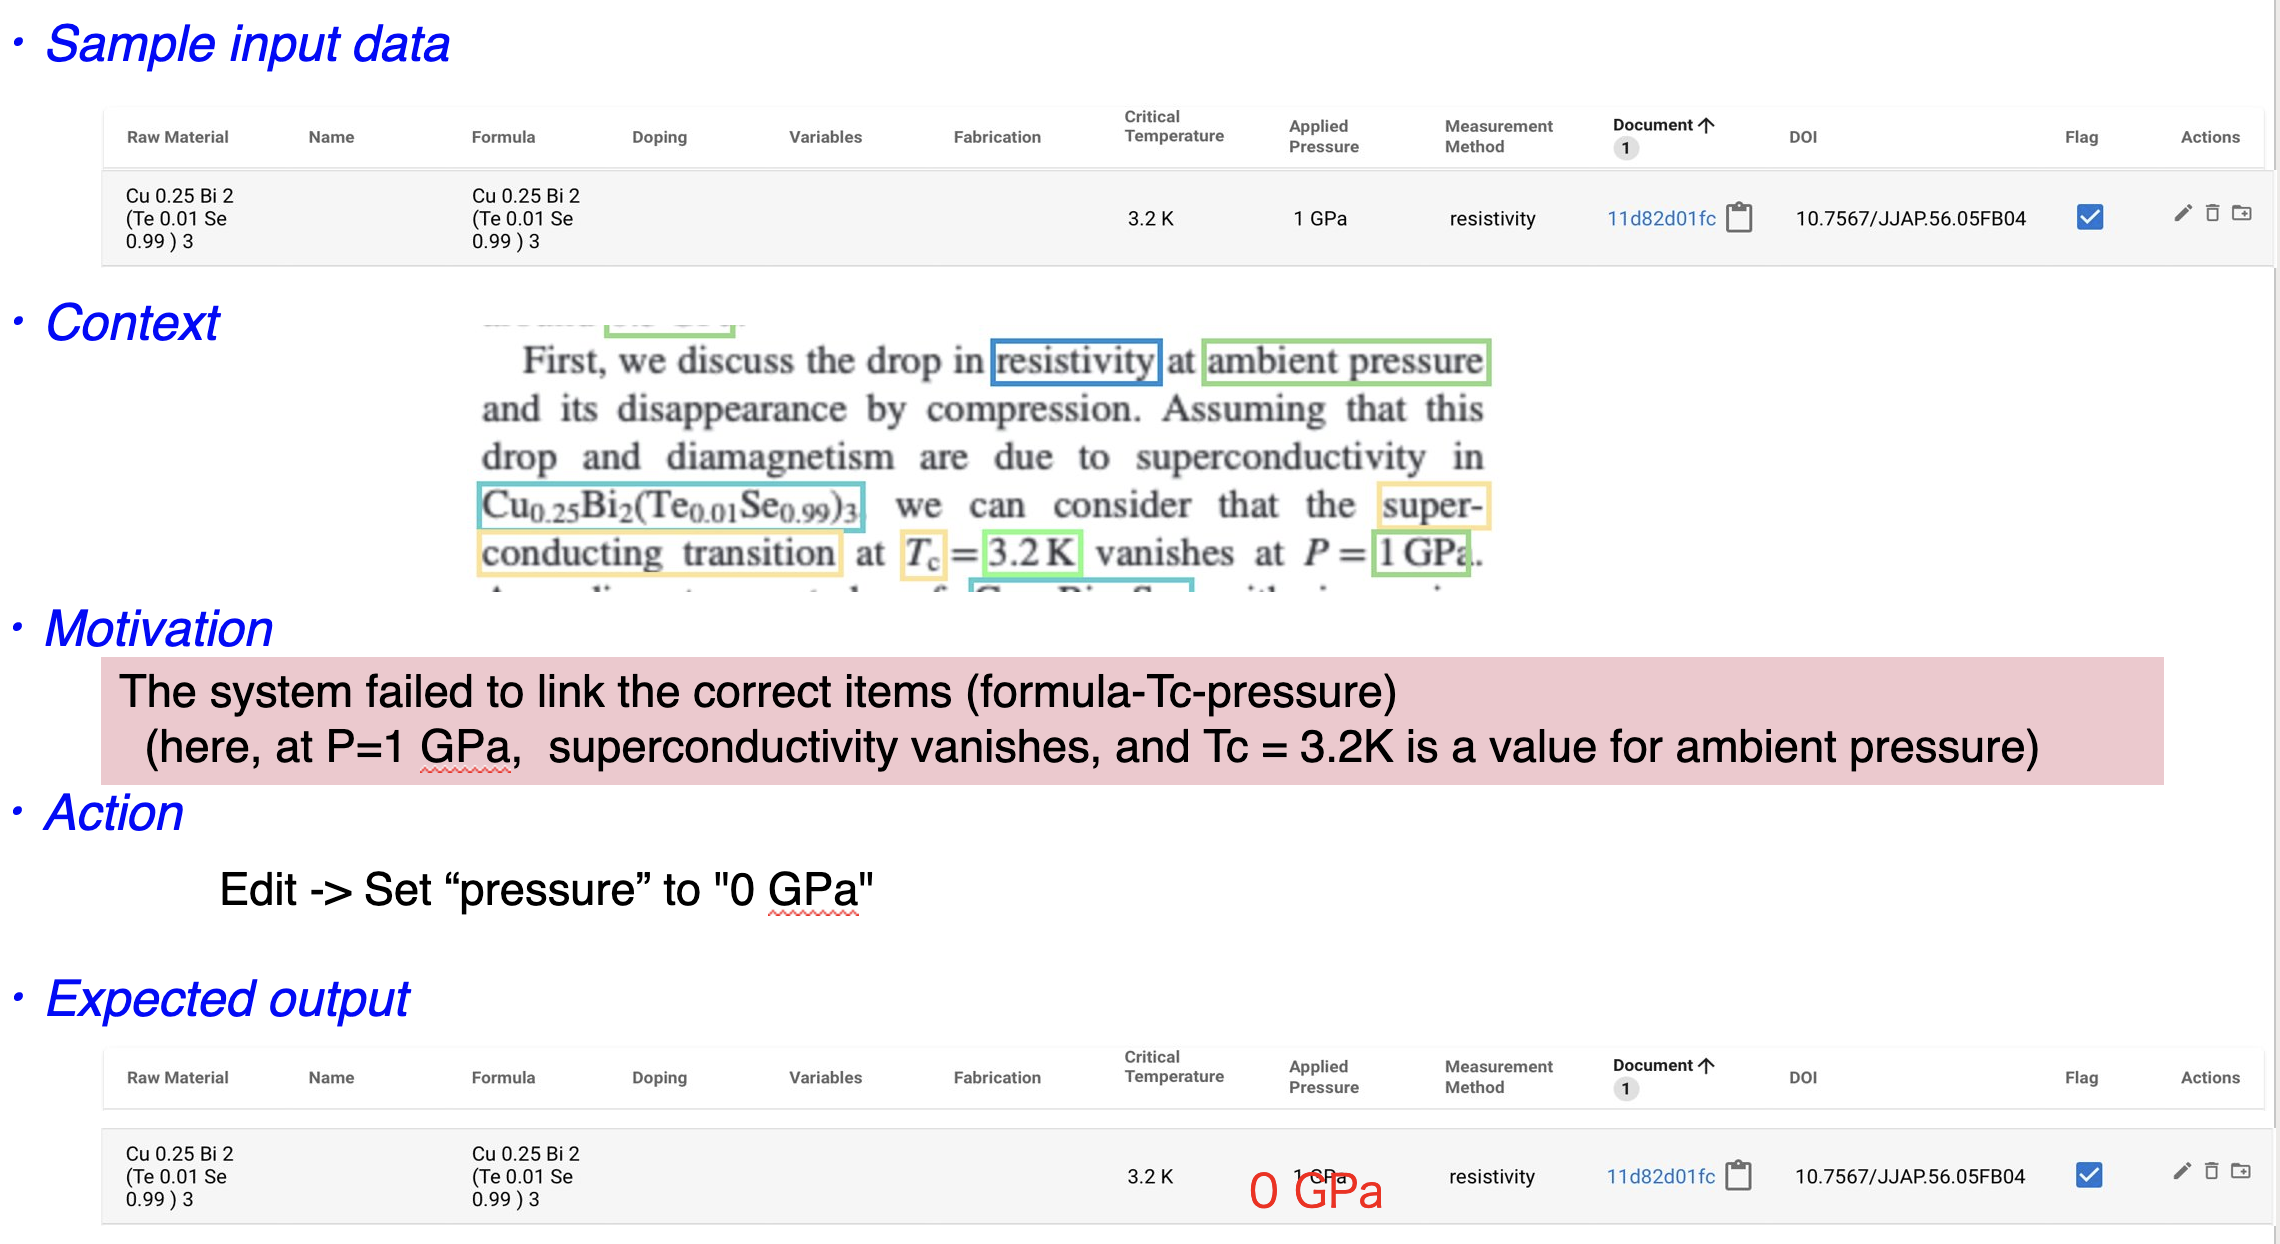
\includegraphics[width=1\textwidth]{images/example-sheet-curation.png} 
  \caption{Example of curation sheet. As discussed, it's written with a simple language assuming the curator may not be familiar with the task. }
  \label{fig:example-curation-sheet}
\end{figure}

\subsection{Feedback loop training data creation}
\label{subsec:feedback-loop-training-data}
One of the key hidden features of this interface is the possibility to generate training data automatically, every time a record is corrected. 

The process works in the following way, when a correction is performed:
\begin{itemize}
    \item the new record with updated information is prepared and stored, 
    \item if the training data exists (e.g. another correction within the same sentence was already performed), then the process finishes
    \item using the record document identifier (the hash), the latest annotation document is retrieved
    \item using the record "materialId" the entity annotation is searched within the annotation document,
    \item when the material is found the passage object containing the text, spans, tokens and other information are collected and saved in a separate collection. The record id is also attached to the training data 
\end{itemize}

The training data can be inspected in a specific page of the application (Figure~\ref{fig:training-data-view}) and sent to the training data annotation tool. We integrated our interface with label-studio~\cite{Label_Studio} which is an open-source and flexible interface. 
Examples are visualised by rows with their document hash and the status which can be "new" when the data is just added or "in progress" after the data is sent to the label-studio application. 
The workflow does not require additional states, because the data can be exported from label-studio after corrected. 


\begin{figure}[ht]
  \centering
  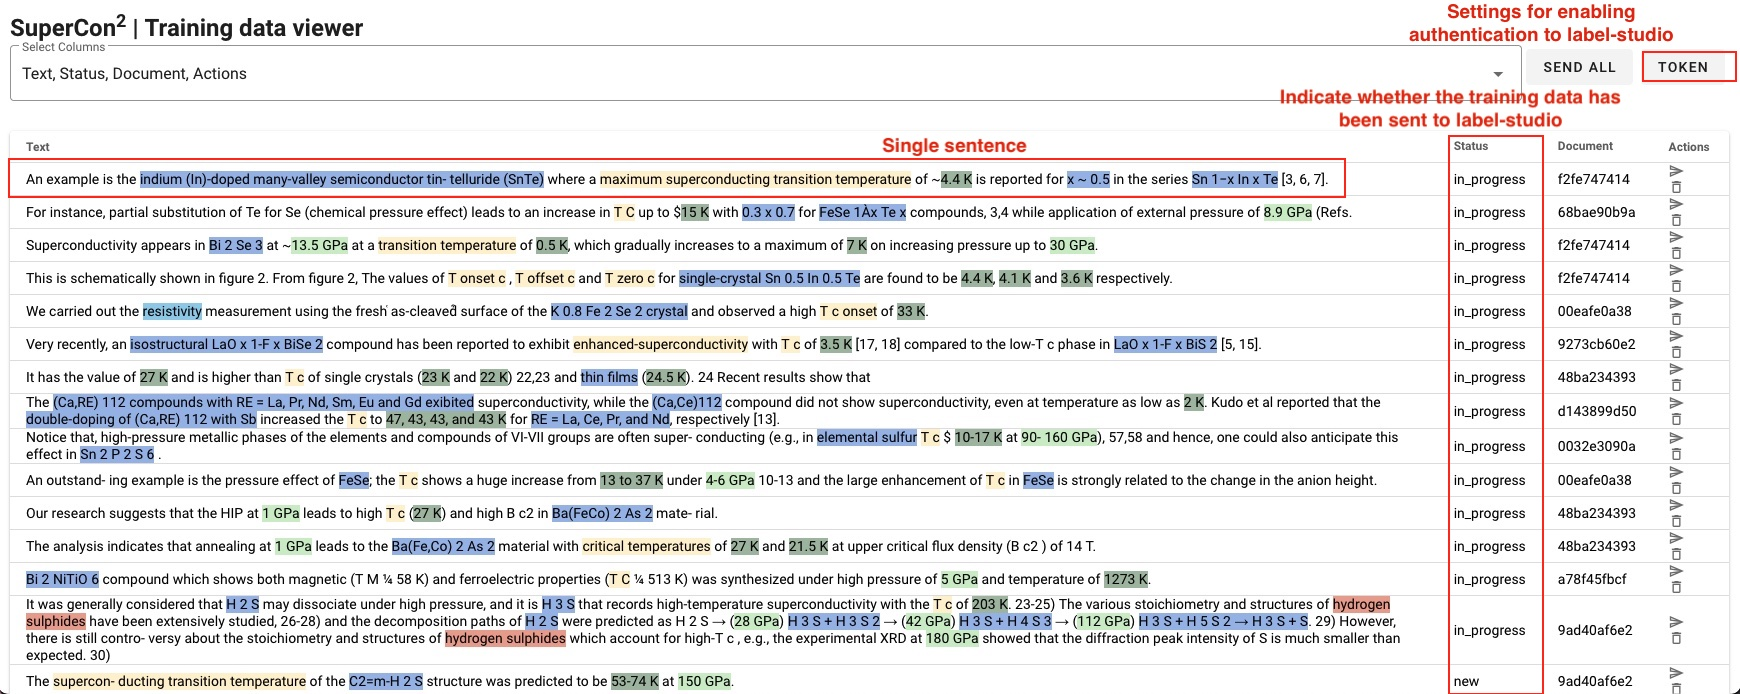
\includegraphics[width=1\textwidth]{images/training-data-viewer} 
  \caption{Training data view}
  \label{fig:training-data-view}
\end{figure}

Since the training data generated with this interface are related to proven mistakes in the TDM process, intuitively they should provide a higher impact in improving the model than training data of the same amount, randomly selected.
To prove this hypothesis, we performed an experiment: we selected around 400 training examples initially marked as incorrect by the anomaly detection script and we curated them. 
Then, we collected the training data and manually correct them, keeping only training data that was actually corrected composing a set of 352 examples. We define \textit{curation} the dataset from curated data and \textit{base} the original SuperMat.

In this experiment we focused on the best model which is based on SciBERT, and that can be trained with two different strategies: "from scratch" when the model is initialised randomly (s) or "incremental" when the initial model weights are used from a trained model (i).
We defined three scenario: a) base from scratch, b) base+curation from scratch, and c) base+curation incrementally. 
We merge curation with the base dataset because the curation dataset is very small as compared with base, to avoid forgetting previous weights.  

The obtained models are tested using a fixed holdout dataset we have designed in our previous work~\cite{lfoppiano2023automatic} and the evaluation scores are illustrated in Table~\ref{tab:evaluation-curation-training}.

\begin{table}[ht]
\centering
\begin{tabular}{|l|l|l|l|}
\hline
& \textbf{Base} & \textbf{base+curation(s)} & \textbf{base(s)+curation(i)} \\ 
\hline
\hline
Nb total examples & 16902 & 17254 & 16902(s), 17254 (i)\\ 
\hline
\texttt{<class>}        & 70,22             & 72,30             & \textbf{72,63} \\ 
\texttt{<material>}     & 79,69             & 80,23             & \textbf{80,61} \\ 
\texttt{<me\_method>}   & 64,78             & 65,31             & \textbf{66,62} \\ 
\texttt{<pressure>}     & \textbf{46,96}    & 46,53             & 46,84 \\ 
\texttt{<tc>}           & 77,36             & 78,56             & \textbf{79,57} \\ 
\texttt{<tcValue>}      & 77,26             & \textbf{77,94}    & 77,84 \\ 
\hline
\textbf{All (micro avg.)} & 75,86           & 76,66             & \textbf{77,36} \\ 
\hline
\textbf{Diff avg. w/ baseline}& -           & +0,80             & \textbf{+1,50} \\ 
\hline
\end{tabular}
\caption{Evaluation scores and comparison of fine-tuning training of SciBERT. The Base dataset is the original dataset described in~\cite{lfoppiano2023automatic}, the curation dataset is automatically collected based on the database corrections by the interface and manually corrected. \textit{s} indicate "training from scratch", while \textit{i} indicate "incremental training". The results are the average of 5 repeated train/eval runs. }
\label{tab:evaluation-curation-training}
\end{table}

The result of this experiment is that with only 352 examples (0.002\% of the SuperMat dataset) we obtained an improvement of +1.50\% F1 score. The incremental approach obtained almost twice the improvement of the model trained from scratch with the extended dataset. 
There are several hypothesis for this, one could argue that the dataset is not big enough for the task at hand, therefore the model requires more training time. This issue could be verified by correcting all the available training data and repeat this experiment. 


\section{Code availability}
This application is freely available at \url{https://github.com/lfoppiano/supercon2}, the repository contains:
\begin{itemize}
\item the code of the SuperCon 2 curation interface for visualising and editing material and properties extracted from superconductors-related papers.
\item The ingestion workflow to create process PDF documents with grobid-superconductors and produce a database of materials and properties.
\item the guidelines, accessible at \url{https://supercon2.readthedocs.io}
\end{itemize}

\section{Acknowledgements}
Our warmest thanks to Patrice Lopez, the author of Grobid~\cite{GROBID}, DeLFT~\cite{DeLFT}, and other open-source projects for his continuous support and inspiration with ideas, suggestions, and fruitful discussions.
We thank Pedro Baptista de Castro for his support during this work. 

\section{Conclusions}
We built a staging area for SuperCon where the data automatically extracted can be examined and corrected by curators in an efficient manner. Thanks to visual aid and contextual connections we improve the quality of curators and their throughput, while providing an efficient system for updating the SuperCon database. 
We demonstrated that the feedback loop based on corrected data can improve substantially the machine learning models with fresh and targeted training data. 

There are several planned features and improvements in the pipeline. Some of these include:

\begin{itemize}
    \item Undo/redo functionality: The ability to undo and redo changes made to records will be added, to make it easier to correct mistakes.
    \item Document versioning: A versioning system will be implemented to track changes to documents over time.
    \item Improved search: The search functionality will be improved to make it easier to find records based on specific criteria.
    \item Additional record types: SuperCon 2 currently supports records for material and property information, but additional record types will be added in the future.
\end{itemize}

\section*{Contributions}
LF wrote the paper and everybody else revised it. 
LF and POS discussed the ML results and designed the various experiments. 
LF wrote the back-end, TM wrote the front-end of the user interface. 
KT lead the materials-science work on the data with CS, TT and WS.
TA revised the paper from CS perspective.
YT and MI supervised the work. 


\bibliography{references}
\bibliographystyle{plain}

\end{document}



